
 \chapter{Spin chains}\label{ch:SpinChains}
 
 \section{Motivation and Introduction}\label{sec:intro2}
 
Many-body systems are usually quite difficult or even impossible to solve analytically due to the insurmountable difficulties in the calculations associated with the staggering number of degrees of freedom a system has. Nonetheless, quantum spin chain models are a class of (often) integrable systems in 1 spatial dimension with very rich physics. The paradigmatic spin chain model is the Heisenberg model introduced simultaneously by Paul Dirac and Werner Heisenberg, hence its name, in 1928 \cite{Heisenberg1928}. It is a model of interacting quantum spin-$1/2$ particles in a one-dimensional lattice conceived as a model for ferromagnetism. This model has critical points where it exhibits quantum phase transitions, analogous to classical phase transitions but at temperature $T=0$. This fact makes it a very interesting model to study. The spin-$1/2$ Heisenberg model in one dimension was first solved by Hans Bethe in 1931 \cite{Bethe1931} by using a plain wave ansatz known as the Bethe ansatz.\\

Of particular interest in this thesis is a special case of the Heisenberg model, the one-dimensional XY-model. This model has a very interesting phase diagram with two quantum phase transitions from separate universality classes, the Ising universality class with central charge $c=1/2$ and the Heisenberg universality class with central charge $c=1$. A solution of the model without a transverse magnetic field was first presented in a seminal paper by Lieb, Mattis and Schultz \cite{Lieb1961407} in 1961, and shortly after the solution with a transverse magnetic field was presented by Neimeijer and Ruijgrok \cite{RUIJGROK1976336}. After the Neimeijer and Ruijgrok in a titanic series of papers, Barouch and McCoy solved the statistical mechanics of the model completely \cite{BM1,BM2}, cementing this model as the paradigmatic physical system for studying quantum phase transitions and quantum dynamics. In recent years, however, the XY-model is being studied in the context of entanglement dynamics and out of equilibrium dynamics within the quantum information science community \cite{vidal,Bennett2000}.\\

In this chapter, we present the solution of the XY-model and compute its spectrum analytically. We follow the usual procedure of first introducing Jordan-Wigner transformation, followed by a Fourier transform and finally a Bogoliubov rotation. We study the structure of the ground state and discuss the model's very rich phase diagram. Additionally, we make special emphasis on the case where the model reduces to the XX-model since it will be key in the next chapter. We discuss the XX-spectrum, its ground state and compute the ground state energy density in the thermodynamic limit.\\

The reader might be wondering why we will make a detour and devote a full chapter to the solution of the XY-model when the title of this thesis makes no mention to spin chains or the XY-model. However, this will be done as to freely borrow results from the solution of the XY-model throughout the following chapter. Why will we need this results in future chapters will become clear shortly, however, at this stage we can say that the discrete form of the Dirac equation yields, under certain conditions, a Hamiltonian equivalent to the XX-model.
 

\section{The XY-model in a transverse field}\label{sec:XYmodel}

The XY-model is a one-dimensional quantum many-body model and a special case of the Heisenberg spin chain model. It is described by the Hamiltonian

\begin{equation}
H(\gamma,g) = J \sum_{n=1}^ N\qty[\frac{1+\gamma}{2}\sigma^x_n\sigma^x_{n+1} +\frac{1-\gamma}{2}\sigma^y_n\sigma^y_{n+1} ] - \frac{g}{2}\sum_{n=1}^N\sigma^z_n\label{eq:XYHam}
\end{equation}

where $0\leq\gamma\leq 1$ is known as the anisotropy parameter. We can choose $\gamma=0$ yielding the isotropic XX-model or $\gamma=1$ yielding the transverse field Ising model. The sign of the coupling $J$ determines whether the chain is ferromagnetic ($J<0$), i.e. the spins tend to align, or antiferromagnetic ($J>0$)  and the spins tend to be anti-aligned. The standard way to tackle a Hamiltonian like \eqref{eq:XYHam} is to map the spin-$1/2$ operators to a set of spinless fermionic operators using a Jordan-Wigner transformation

\begin{align}
\sigma_n^x &= \qty[\prod_{l<n}\sigma^z_l](\phi_n^\dagger + \phi_n)\nonumber\\
\sigma_n^y &= i\qty[\prod_{l<n}\sigma^z_l](\phi_n^\dagger - \phi_n)\\
\sigma_n^z &= (1-2\phi_n^\dagger \phi_n )\nonumber
\end{align}


such that the set $\{\phi_n\}_{n=1,\ldots,N}$ obeys the usual CAR algebra

\begin{equation}
\{\phi_i, \phi_j^\dagger\}= \delta_{ij} \quad \{\phi_i, \phi_j\}=\{\phi_i^\dagger, \phi_j^\dagger\}=0.
\end{equation}

By virtue of the Jordan-Wigner transformation, the eigenstates of $\sigma^z$, $\ket{\uparrow}$ and $\ket{\downarrow}$ are mapped into $\ket{0}$ and $\ket{1}$, which represent the presence or absence of a fermion in each lattice site. Applying the transformation to Hamiltonian \eqref{eq:XYHam} yields

\begin{equation}
    H(J,\gamma,g) = J\sum_{n=1}^{N}\qty[\phi^\dagger_n  \phi_{n+1} + \phi^\dagger_{n+1}\phi_n + \gamma\qty(\phi_n^\dagger\phi^\dagger_{n+1} + \phi_{n+1}\phi_n)] + 2g\sum_{n=1}^{N}\phi_n^\dagger\phi_n - \frac{gN}{2}.
\end{equation}

We can ignore the constant term $gN/2$ since it is a simple energy offset that is irrelevant to the physics of the system.\\

 This Hamiltonian can be diagonalized using a combination of Fourier and Bogoliubov transformations. First, let us introduce the momentum representation of the fermionic operators, namely

\begin{equation}
\phi_k  = \frac{1}{\sqrt{N}}\sum_l \phi_l e^{-i k_n l};\quad k_n= \pi\qty(\frac{2n +1}{Na}),\quad n = 0,\pm 1,\ldots,\pm N, \label{eq:kn}
\end{equation}

Where $a$ is the lattice spacing. The momentum $k_n$ lies in the set $[-\pi/a , \pi/a]$. Additionally, the condition that the Fourier transformed operators satisfy the CAR algebra plus the condition of being in the even parity sector (as we are interested in the ground state) fixes the values of the $k_n$'s in \eqref{eq:kn}. In the Fourier basis, the Hamiltonian can be neatly written as the almost diagonal form

\begin{equation}\label{eq:FourierHam}
    H(J,\gamma,g)  = \sum_{k>0}\qty[\qty(g - J\cos k_n)\phi_k^\dagger\phi_k - iJ\gamma\sin{k_n}\qty(\phi_k^\dagger\phi_{-k}^\dagger + \phi_k\phi_{-k})],
\end{equation}

which is equivalent to the matrix form

\begin{equation}
H(J,\gamma,g) = \sum_k (\phi_k^\dagger,\,\phi_{-k}) \mqty(\alpha(k_n)& -i\beta(k_n) \\ i\beta(k_n) & -\alpha(k_n))\mqty(\phi_k\\\phi_{-k}^\dagger),
\end{equation}

with $\alpha(k_n) = g-J\cos(k_n)$ and $\beta(k_n) = J\gamma\sin(k_n)$. This form of the Hamiltonian suggests that in order to diagonalize it we should make use of a Bogoliubov transformation that only mixes $\phi_k^{\dagger}$ with  $\phi_{-k}^{\dagger}$. Hence, the correct transformation is

\begin{equation}
\eta_k = u_k(\gamma,g)\phi_k - i v_k(\gamma,g)\phi_{-k}^\dagger,\quad\eta _{-k}=u_k(\gamma,g)\phi_{-k} + i v_k(\gamma,g)\phi_{k}^\dagger
\end{equation}

where the $\eta_k$ represent the new Bogoliubov fermions. The old fermions are given in terms of the inverse transformation

\begin{equation}
\phi_k =  u_k(\gamma,g)\eta_k + i v_k(\gamma,g)\eta_{-k}^\dagger,\quad \phi _{-k}=u_k(\gamma,g)\eta_{-k} - i v_k(\gamma,g)\eta_{k}^\dagger.
\end{equation}

The transformation coefficients $u(\gamma,g),v(\gamma,g)$ being real and the unitarity of the transformation enforces the conditions that $u_k^2(\gamma,g) + v_k  ^{2}(\gamma,g)=1$.  This fact suggests to us the parametrization

\begin{equation}
u_k(\gamma,g)  = \cos(\frac{\theta_k}{2} ),\quad v_k(\gamma,g) = \sin(\frac{\theta_k}{2}).\label{eq:paramBogo}
\end{equation}

Applying the transformation yields the following Hamiltonian

\begin{multline}
H(J,\gamma,g) =\\
 \sum_k (\phi_k^\dagger,\,\phi_{-k}) \mqty(u_k & iv_{-k}\\-iv_k & u_{-k} )\mqty(\alpha(k_n)& -i\beta(k_n) \\ i\beta(k_n) & -\alpha(k_n))\mqty(u_k & iv_{-k}\\-iv_k & u_{-k} )^{-1}\mqty(\phi_k\\\phi_{-k}^\dagger).
\end{multline}

The objective of applying the Bogoliubov rotation is to make the off-diagonal terms vanish, and as such enforcing the requirement that the coefficients of the off-diagonal terms vanish leads to the condition

\begin{equation}
    \frac{u_k v_k}{u_k^2 + v_k^2} =  \frac{J\gamma\sin(k_n)}{g-J\cos(k_n)},
\end{equation}

provided that both $u_k$ and $v_k$ are eigenstates of the Bogoliubov- de Gennes equations

\begin{align}
   \mqty(\alpha(k_n)& -i\beta(k_n) \\ i\beta(k_n) & -\alpha(k_n))\mqty(u_k\\v_k) = \epsilon_k \mqty(u_k\\v_k)\label{eq:BdG}.
\end{align}

Equation \eqref{eq:BdG} implies there are two eigenstates for each $k$ with single particle energies given by


\begin{equation}
    \epsilon_k = \pm \sqrt{(g- J\cos(k_n))^2 + (J\gamma \sin(k_n))^2}.\label{eq:XYspectrum}
\end{equation}




Note that applying the Bogoliubov transformation together with the parametrization \eqref{eq:paramBogo} diagonalizes the Hamiltonian provided that the Bogoliubov angles satisfy 

\begin{align}
        \tan(\theta_k) &= \frac{J\gamma\sin(k_n)}{g-J\cos(k_n)}\nonumber\\ 
        \sin(\theta_k) &= \frac{J\gamma\sin(k_n)}{\sqrt{(g- \cos(k_n))^2 + (J\gamma \sin(k_n))^2}}\\
        \cos(\theta_k) &= \frac{g - J\cos(k_n)}{\sqrt{(g- \cos(k_n))^2 +  (J\gamma \sin(k_n))^2}}\nonumber,\label{eq:BogoCond}
\end{align}

or equivalently

\begin{equation}
    e^{i \theta_k} = \frac{g-J\cos k_n + iJ\gamma \sin k_n}{\sqrt{(g-J\cos k_n)^2 + (J\gamma\sin k_n)}}.
\end{equation}

Choosing the positive energy eigenstate from \eqref{eq:XYspectrum} the Hamiltonian is written as a diagonal form in terms of the Bogoliubov fermions, viz

\begin{equation}\label{eq:dHamil}
H = \sum_k\epsilon_k\qty(\eta_k^\dagger\eta_k -\frac{1}{2}).
\end{equation}


\subsection{The ground state}\label{ssec:groundstate}

The ground state (or Bogoliubov vacuum) of the Hamiltonian \eqref{eq:dHamil} will be labeled $\ket{\rm{GS}}$. Having brought the Hamiltonian to the diagonal form, the ground state will be given by the condition

\begin{equation}
    \eta_k \ket{\rm{GS}} = 0\quad \forall k.
\end{equation}

 However, let us consider the ``vacuum'' state $\ket 0$ for the $\phi$-fermions, which is defined by the condition 
 
 \begin{equation}
     \phi_k\ket 0 = 0\quad \forall k.
 \end{equation}
 
Let us note that we can define 

\begin{equation}
B_k \overset{.}{=} u_k(g)+ iv_k(g)\phi_k^\dagger \phi_{-k}^\dagger
\end{equation} 

with $u_k(g)$ and $v_k(g)$ the Bogoliubov coefficients \eqref{eq:paramBogo}. Moreover, this definition implies that $$\phi_k B_k\ket 0_\phi = 0.$$ Therefore, we can rewrite the ground state as a product of all the different $B_k$'s, viz

\begin{equation}
\ket{\rm{GS}} = \prod_{k>0} \qty(u_k(g)+ iv_k(g)\phi_k^\dagger \phi_{-k}^\dagger)\ket 0_\phi.\label{eq:gsB}
\end{equation}

Hence, equation \eqref{eq:gsB} tells us that $\ket{\text{GS}}$ contains an even number of $\phi$-fermions that are always created as particle pairs with momenta $(k,-k)$.

\subsection{The Phase Diagram}\label{ssec:PhaseDiag}

The zero temperature phase diagram of the XY-model in parameter space $(\gamma,g)$ is depicted in figure \ref{fig:PhaseDiagram}. It is interesting to note that we can identify several critical regions of the parameter space where the spectrum \eqref{eq:XYspectrum} is zero. In particular, this implies that the gap vanishes and low energy quasi-particles dominate the behavior of the system. 

\begin{figure}[htb]
	\centering
	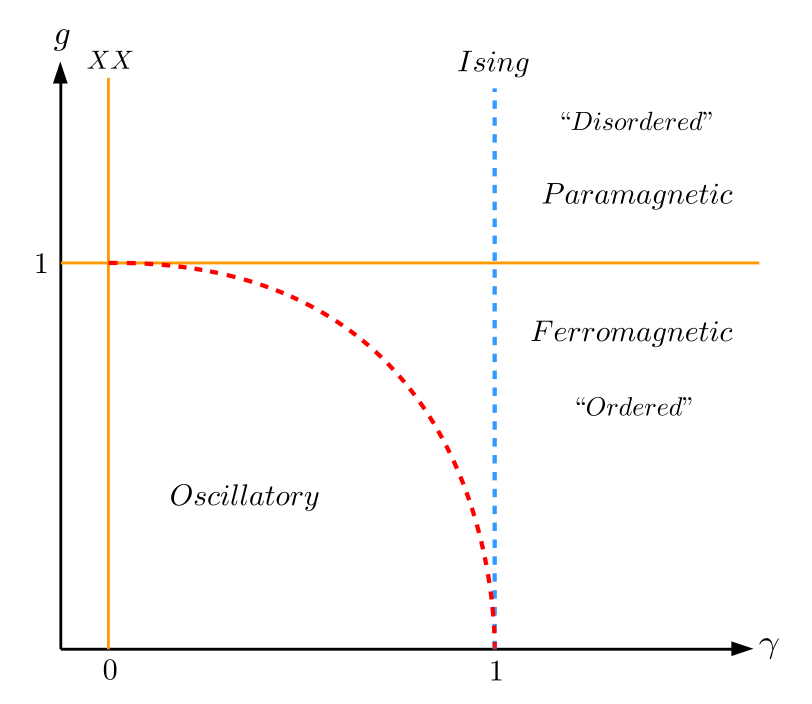
\includegraphics[scale=0.45]{figures/XYPhase.png}
	\caption{Phase diagram of the XY-model for $\gamma$ and $g$ positive.}
	\label{fig:PhaseDiagram}
\end{figure}

Figure \ref{fig:PhaseDiagram} shows the critical lines, $\gamma=0$ which corresponds to the isotropic XY-model more commonly known as the XX-model. The line $g=1$ is a critical line of the XY-model due to the transverse magnetic field. At the intersection of this line with the line $\gamma=1$ lies the critical point of the transverse field Ising model. Below the $g=1$ line the ground state is a doubly degenerate having a $\mathbb{Z}_2$ symmetry. In the ferromagnetically ordered phase $g<1$, this  $\mathbb{Z}_2$ symmetry is broken yielding a two-fold degeneracy in the ground state given by two states of opposite longitudinal magnetization

\begin{align}
	\ket{\psi_1} &= \ket{\rightarrow\ldots\rightarrow}=\prod_{l=1}^{N}\frac{1}{\sqrt{2}}\qty[\ket\uparrow _l + \ket\downarrow_l],\nonumber\\ 
	\ket{\psi_2} &= \ket{\leftarrow\ldots\leftarrow}= \prod_{l=1}^{N}\frac{1}{\sqrt{2}}\qty[\ket\uparrow _l - \ket\downarrow_l] .
\end{align}


The region $g>1$ has a single ground state where all the spins are aligned with the transverse field. Finally, the line defined by $\gamma^2 + g^2 = 1$ corresponds to a region where the ground state wavefunction can be written aa product over single spin states.


\section{The XX-model}\label{sec:XXmodel}

The XX model corresponds to the special case of the XY-model when $\gamma = 0$. In which case the Hamiltonian is already diagonal after the Fourier transform as seen from equation \eqref{eq:FourierHam}. Thus, the Hamiltonian for the XX model after the Fourier transform reads

\begin{equation}\label{eq:XXHam}
H_{XX}(J,g)  = \sum_{k>0}\qty(g - J\cos k_n)\phi_k^\dagger\phi_k,
\end{equation}

from which we can immediately read the single particle energy dispersion relation to be

\begin{equation}
\epsilon_k = g-J\cos(k_n).
\end{equation}

\begin{figure}[htb]
	\centering
	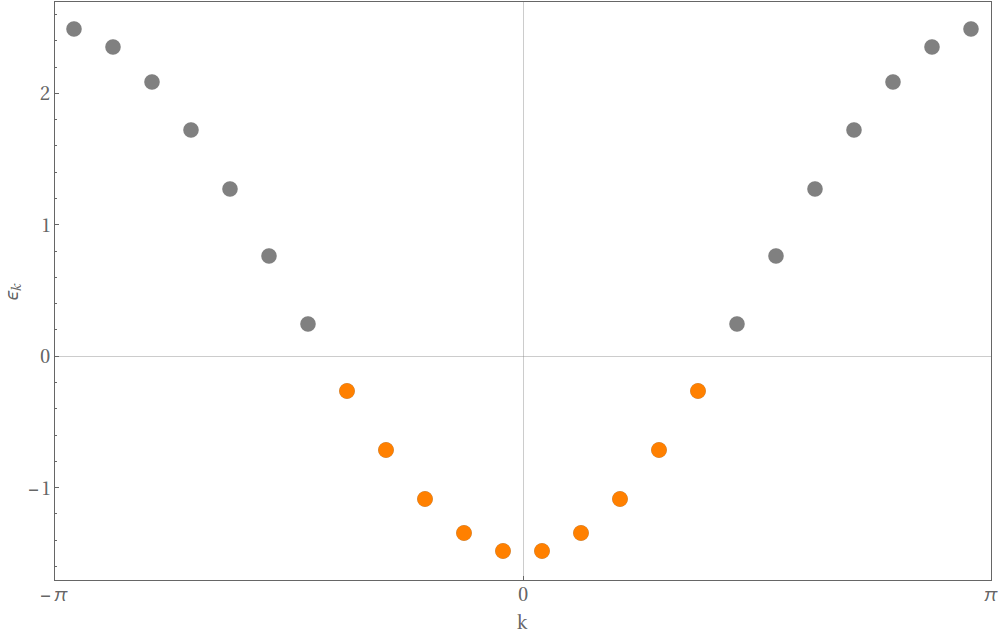
\includegraphics[scale=0.35]{figures/XXSpectrum.png}
	\caption{$N=24$ XX-model spectrum for $g=1/2$ and $J=1$. The orange dots are filled Dirac sea states of the ground state.}
	\label{fig:XXSpec}
\end{figure}

The single particle energy spectrum is shown in figure \ref{fig:XXSpec}. For $g>J$ the spectrum is positive and the ground state contains no fermions. However, for $J>g$ the spectrum has negative energy states corresponding to fermions with $k<|\cos^{-1}(g/J)|$.\\

The standard procedure is to fill the negative energy states, i.e. the Dirac sea in order to define the ground state of the system

\begin{equation}
\ket{\text{GS}} = \prod_{k<\abs{\cos^{-1}\qty(\frac{g}{J})}}\phi^\dagger_k\ket{0},
\end{equation}

with $\ket{0}$ being the vacuum state of the fermions. This ground state corresponds to a spin chain with a half-filled band. Excited states above the ground state in this spin system correspond to adding a fermion with $k>\abs{\cos^{-1}\qty(g/J)}$ or annihilating one with $k<\abs{\cos^{-1}\qty(g/J)}$ to form a hole. \\

In the limit $N\to\infty$ we can compute the ground state energy per spin by replacing summations with integrals

\begin{equation}
\frac{E_0}{N} = -\frac{1}{2}\sum_k|\epsilon_k|\to \frac{E_0}{N} = -\frac{1}{2}\int_{-\pi}^{\pi}\frac{\dd{k}}{2\pi}\dd{k}|\epsilon_k|,
\end{equation}

which after integration yields

\begin{equation*}
	\frac{E_0}{N} =-\frac{2 \sqrt{1-g^2}+\pi  g-2 g \cos^{-1}(g)}{2 \pi }.
\end{equation*}

For the special case of zero transverse field, $g=0$ the ground state energy reduces to

\begin{equation}
\frac{E_0}{N} = -\frac{1}{\pi}
\end{equation}

This value will be very useful to us in the next chapter as we will use it as a benchmark in the various computer simulations of the model.

\section{Comments and conclusion}\label{sec:conclusion2}

Throughout this chapter, we have delved into the complete analytical solution of the XY-model in a transverse field. The solution presented in this chapter is the standard solution where the spin Hamiltonian is first mapped to a spinless fermion Hamiltonian by means of the Jordan-Wigner transformation. After the Jordan-Wigner transformation and taking advantage of the translation symmetry of the system, we diagonalized the Hamiltonian by introducing a Fourier transform followed by Bogoliubov rotation. This combination of unitary transformations fully diagonalized the fermion Hamiltonian. In this diagonal form, we find the single particle spectrum of the model to be 

\begin{equation*}
	\epsilon_k =  \sqrt{(g- J\cos(k_n))^2 + (J\gamma \sin(k_n))^2}.
\end{equation*}

Additionally, by inspecting the ground state written in terms of the Fourier transformed fermions, we found that it is a state always composed by pairs of quasiparticle with opposite momenta

\begin{equation*}
	\ket{\rm{GS}} = \prod_{k>0} \qty[\cos\qty(\frac{\theta_k}{2})\ket 0_\phi+ i\sin\qty(\frac{\theta_k}{2})\ket{k,-k}].
\end{equation*}

Furthermore, in section \ref{ssec:PhaseDiag} we briefly analyzed the phase diagram of the XY-model (cf figure \ref{fig:PhaseDiagram}). We identified two critical lines, $\gamma=0$ and $\gamma=1$, that correspond to different universality classes, Ising universality, and Heisenberg universality class respectively. Also, we briefly commented on the structure of the ground state in each phase.\\

Finally, during section \ref{sec:XXmodel} we analyzed the XX-model, a special case of the XY-model with $\gamma=0$. We computed its spectrum (cf. figure \ref{fig:XXSpec}) and commented briefly on the structure of its ground state. The ground state had all of the negative energy states are filled following Dirac prescription of filling the Dirac sea. Furthermore, we calculated the ground state energy per spin, which in the special case of no transverse magnetic field reduces to 

\begin{equation*}
	\frac{E_0}{N} = -\frac{1}{\pi},
\end{equation*}

this result will prove useful in the following chapters where the ground state energy of the free Schwinger model will be computed numerically.